\documentclass{beamer}
\usetheme{Berkeley}
\usecolortheme{seagull}
\usefonttheme{serif}
%\usefonttheme{structuresmallcapsserif} %forse un po' troppo pretenzioso

\usepackage[english,italian]{babel}
\usepackage{lipsum}
\usepackage{siunitx}
\usepackage{tikz}
\usepackage{pgfplots}
\usepackage{pgfplotstable}
\pgfplotsset{
	compat=newest,
	every tick label/.append style={font=\scriptsize},
	every node near coord/.append style={font=\scriptsize}
}
\usepgfplotslibrary{ternary}
\usetikzlibrary{calc}
\usepackage{todonotes}
\usepackage{url}
\usepackage[export]{adjustbox}

\title{OpenLDAT}
\subtitle{Un sistema di misurazione di metriche di latenza dei display}
\author{Federico Dossena}
\institute{Università degli Studi di Milano}
\date{2021-??-??}

\begin{document}
	
\begin{frame}
	\titlepage
\end{frame}

\section{Introduzione}
\begin{frame}
	\frametitle{Introduzione}
	\lipsum[1]
\end{frame}
\begin{frame}
\frametitle{Nvidia LDAT (1)}
\begin{itemize}
	\item A Settembre 2020, Nvidia ha inviato dei prototipi di \textcolor{blue}{Nvidia LDAT} a dei giornalisti specializzati, ma non ha poi commercializzato il prodotto
	\item Il dispositivo permetteva di misurare la \textcolor{blue}{latenza totale del sistema} in modo manuale o semi-automatico
	\item Il progetto \textcolor{blue}{OpenLDAT} vuole ricreare questo dispositivo, aggiungere più funzioni, utilizzarlo per testare dei display, e distribuirlo su \textcolor{blue}{licenza libera}.
\end{itemize}
\begin{block}{Latenza totale del sistema}
	Tempo che intercorre tra un'azione nel mondo fisico, come un click del mouse, e la visualizzazione del risultato sul display.
\end{block}
\end{frame}
\begin{frame}
	\frametitle{Nvidia LDAT (2)}
	\centering
	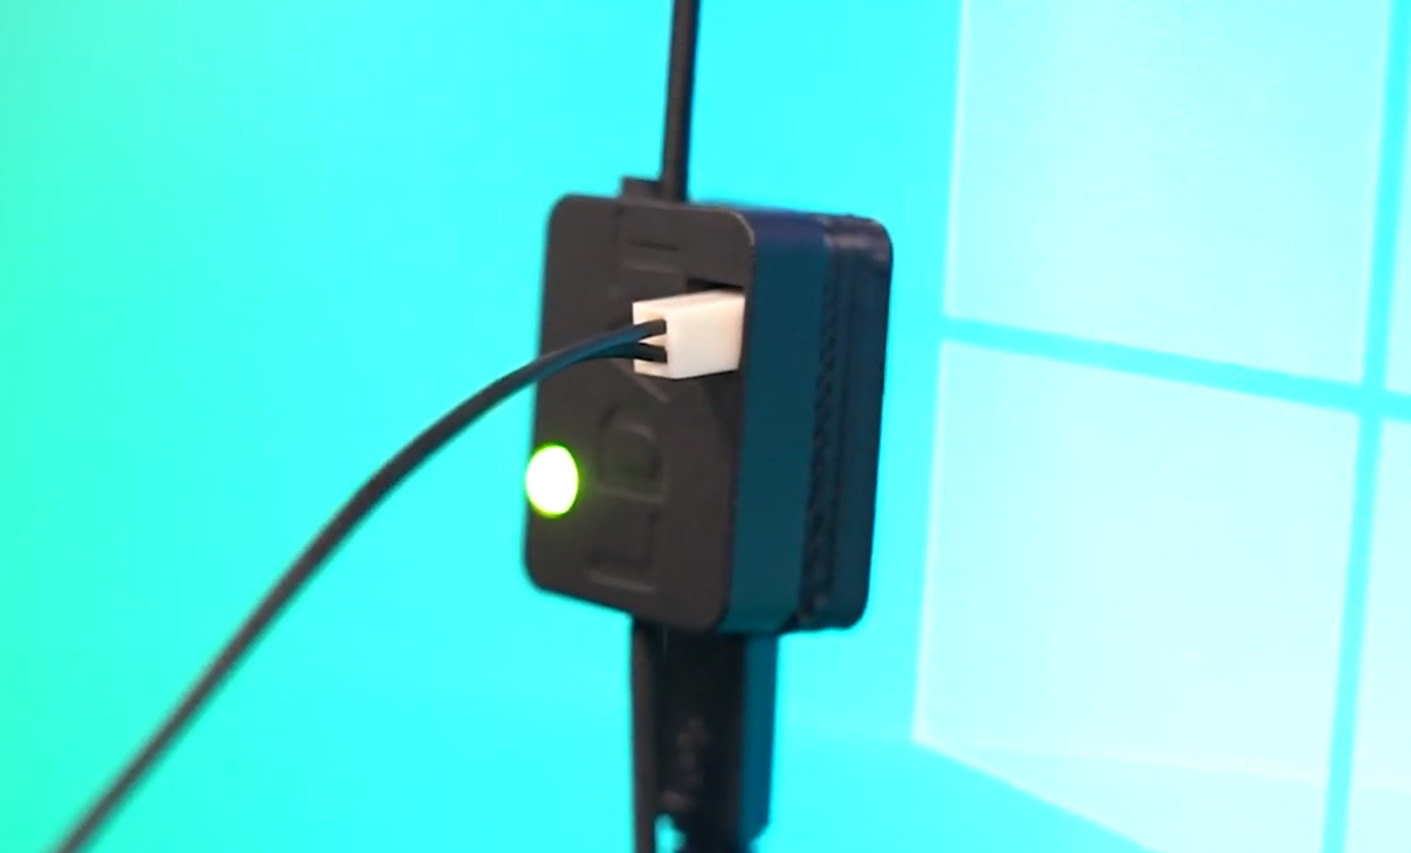
\includegraphics[height=0.45\textheight]{StatoDellArte_files/nvldat_front.jpg}
	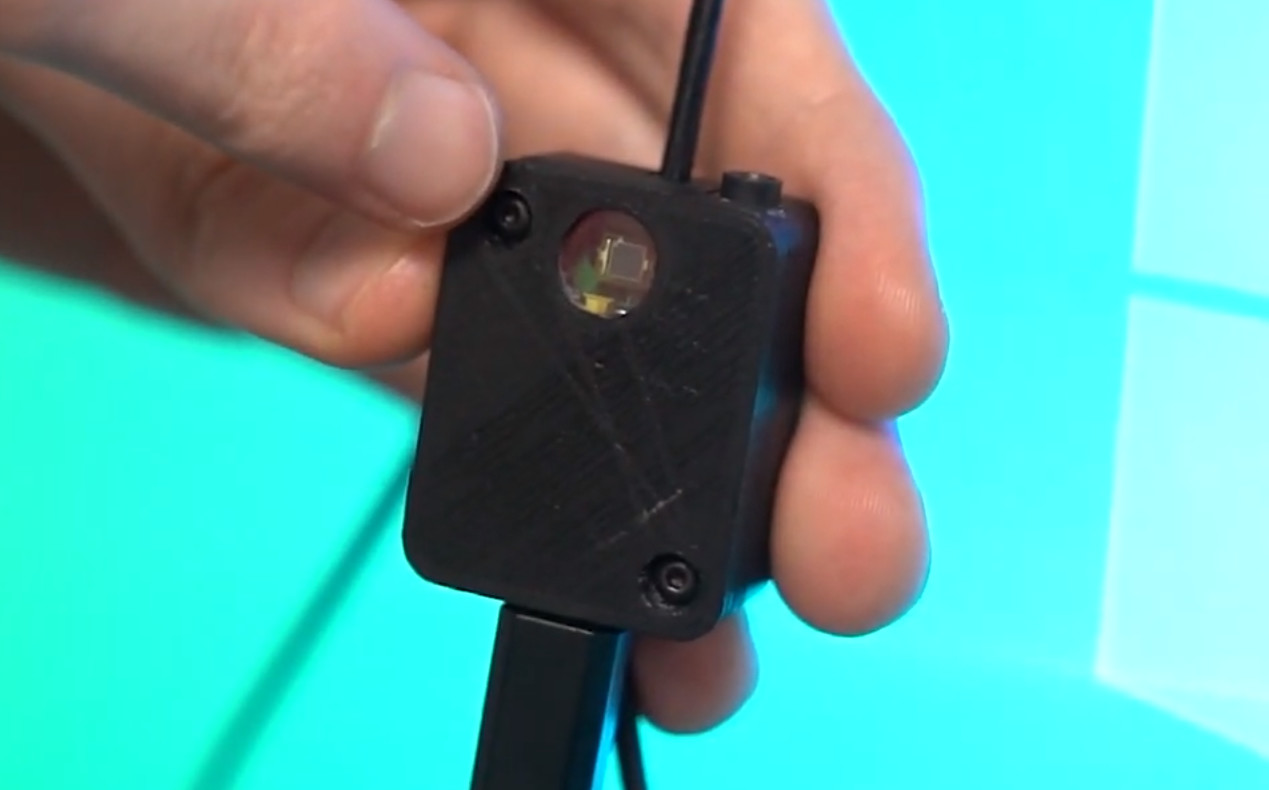
\includegraphics[height=0.45\textheight]{StatoDellArte_files/nvldat_back.jpg}
\end{frame}

\section{Dispositivo}
\begin{frame}
\frametitle{Dispositivo OpenLDAT}
\begin{columns}
	\column{0.5\textwidth}
	\begin{itemize}
		\item Microcontroller \textcolor{blue}{ATmega32U4}
		\item Fototransistor \textcolor{blue}{ALS-PT19}
		\item \textcolor{blue}{PCB} personalizzato
		\item Generazione dei \textcolor{blue}{click automatica o manuale}
		\item \textcolor{blue}{LED per validazione} con telecamera ad alta velocità
		\item Campionamento fino a \textcolor{blue}{\textasciitilde 30kHz 10-bit}
		\item Poco costoso e facile da realizzare
	\end{itemize}
	\column{0.5\textwidth}
	\adjincludegraphics[trim={{.22\width} 0 {.22\width} 0},clip,width=0.6\textheight]{Dispositivo_files/assembly_15.jpg}
\end{columns}
\end{frame}

\section{Applicazione}
\begin{frame}
	\frametitle{Applicazione OpenLDAT (1)}
	\lipsum[1]
\end{frame}
\begin{frame}
	\frametitle{Applicazione OpenLDAT (2)}
	\lipsum[1]
\end{frame}

\section{Risultati sperimentali}
\begin{frame}
	\frametitle{Input lag (1)}
	\lipsum[1]
\end{frame}
\begin{frame}
	\frametitle{Input lag (2)}
	\lipsum[1]
\end{frame}
\begin{frame}
	\frametitle{PWM e noise}
	\lipsum[1]
\end{frame}
\begin{frame}
	\frametitle{Risposta dei pixel}
	\lipsum[1]
\end{frame}
\begin{frame}
	\frametitle{Overdrive}
	\lipsum[1]
\end{frame}
\begin{frame}
	\frametitle{Microstuttering}
	\lipsum[1]
\end{frame}

\section{Conclusioni}
\begin{frame}
	\frametitle{Conclusioni}
	\lipsum[1]
\end{frame}
\begin{frame}
	\frametitle{Grazie per l'attenzione}
	Link al progetto...
\end{frame}

\end{document}
